\documentclass{article}
\setlength{\parskip}{0pt} % esp. entre parrafos
\setlength{\parindent}{3pt} % esp. al inicio de un parrafo
\usepackage{amsmath} % mates
\usepackage{listings}
\usepackage[sort&compress,numbers]{natbib} % referencias
\usepackage{url} % que las URLs se vean lindos
\usepackage[top=10mm,left=20mm,right=20mm,bottom=25mm]{geometry} % \textbf{\textbf{}}margenes
\usepackage{hyperref} % ligas de URLs
\usepackage{graphicx} % poner figuras
\usepackage[spanish]{babel} % otros idiomas
\hypersetup{
    colorlinks=true,
    linkcolor=blue,
    filecolor=blue,      
    urlcolor=blue,
}

\title{TAREA \# 1 \\ Movimiento Browniano} %titulo
\author{Natalia Berenice P\'{e}rez L\'{o}pez} % author
\date{\today}

\begin{document} % inicia contenido

\maketitle % cabecera

\section{Objetivo}
El objetivo de esta práctica es examinar los efectos de la dimensión en la distancia Manhattan del Movimiento Browniano de una partícula para varias dimensiones (en incrementos multiplicativos), variando el número de pasos de la caminata en cuatro niveles (Nivel 1= 20 pasos, Nivel 2= 200 pasos, Nivel 3= 2000 pasos, Nivel 4= 20000 pasos), con 12 repeticiones del experimento para cada combinación. Los resultados se observan en una sola gráfica con diagramas de caja-bigote.

\section{Desarrollo} % seccion y etiqueta
Se realizaron diversos intentos para generar el código objetivo de la práctica, dichos intentos se encuentran en \href{https://github.com/nataliaperez0/Simulation/tree/main/Tarea1/}{mi repositorio}  en GitHub. Inicie tomando como base el \href{https://github.com/satuelisa/Simulation/blob/master/BrownianMotion/brownian.R}{código de Movimiento Browniano} revisado en clase \citep{1}, a este código le quité el paso de evaluar la distancia euclidiana, y para variar la caminata mi primera opcion fue agregar cuatro 'for', para así ejecutar los cuatro niveles de caminata. Así mismo los resultados de cada experimento se almacenaban en un 'data.frame' (Ver Figura 1 \ref{Figura1}) vacío que se colocó al inicio del programa. Con este \href{https://github.com/nataliaperez0/Simulation/blob/main/Tarea1/Pruebas%20de%20codigo/Intento%208.R}{nuevo código}  al final se generó una gráfica con la información del 'data.frame' (Ver Figura 2 \ref{Figura2}).

\begin{figure} [h!]% figura
    \centering
    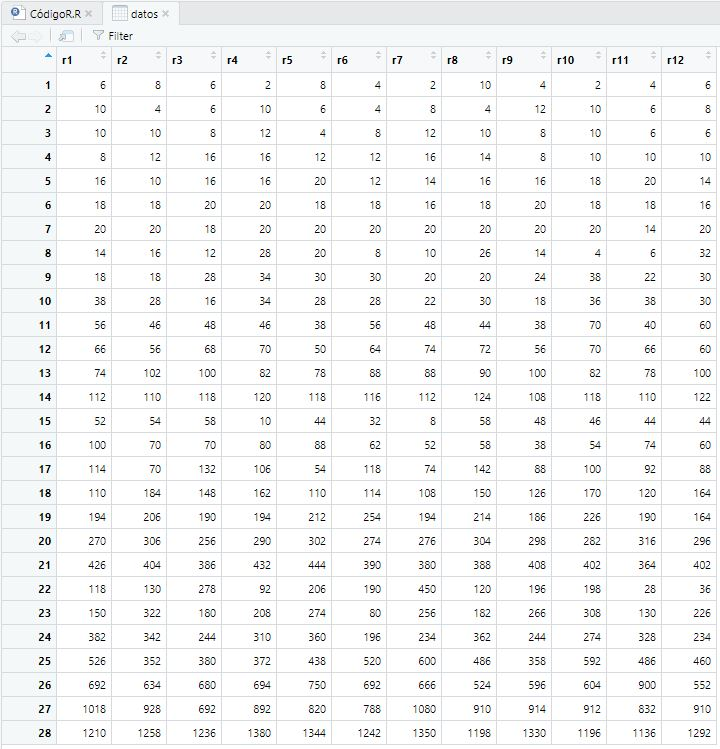
\includegraphics[width=80mm]{Figura1.jpg} % archivo
    \caption{'Data.frame' que se obtiene al ejecutar el programa.}
    \label{Figura1}
\end{figure}

En la Figura 1 \ref{Figura1} podemos ver que las primeras 7 filas corresponden a las distancias de la caminata Nivel 1, de la fila 8 a la 14 corresponden a la caminata Nivel 2, de la 15 a la 21 corresponden a la caminata Nivel 3 y de la 22 a la 28 al Nivel 4. En la  Figura 2 \ref{Figura2} podemos ver que los 4 niveles de caminata se ordenan de manera consecutiva en el 'eje x' debido al ordenamiento de los datos en el 'data.frame'. Ya que la gráfica generada no permite visualizar los datos correctamente, se utilizó la libreria 'ggplot2', la cual permite generar diagramas de caja-bigote agrupados.

\newpage
.
\bigskip
\bigskip

\begin{figure} [h!]% figura
    \centering
    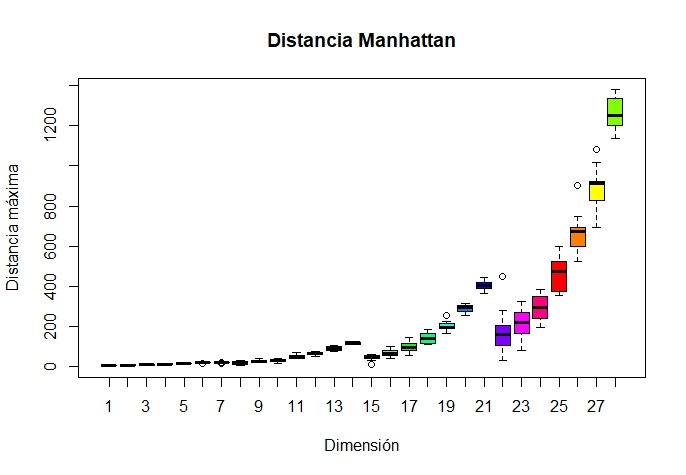
\includegraphics[width=170mm]{Figura2.jpeg} % archivo
    \caption{Primer intento de diagrama caja-bigote para los 4 niveles de caminata.}
    \label{Figura2}
\end{figure}

Se revisaron diferentes páginas en internet sobre documentación \citep{2}, \citep{3} y video tutoriales para aprender a realizar diagramas caja-bigote o boxplot con la librería 'ggplot2'\citep{8}, \citep{9}, \citep{10}, sin embargo debido al ordenamiento que tenia mi 'data.frame' se me dificultó acomodar las variables para generar mi boxplox, ya que en éste se deben indicar los datos para el 'eje x' y los datos para el 'eje y'. Se revisó documentación para tratar ordenar adecuadamente los datos en el 'data.frame' \citep{4}, \citep{5}, \citep{6}, \citep{7}.

\bigskip
El siguiente paso que realicé fue preguntar mis dudas a mis compañeros, y mi compañera de clase Claudia Hernández me explicó una metodología para realizar una gráfica en 'ggplot2', la cual consistía en importar un archivo de Excel con los datos debidamente ordenados y a partir de éste generar el diagrama caja-bigote. De esta forma con mi código obtuve las distancias para los 4 niveles de caminata y los acomode en un archivo de Excel, el cual posteriormente importé y después generé \href{https://github.com/nataliaperez0/Simulation/blob/main/Tarea1/Pruebas%20de%20codigo/Graficar%20con%20Excel%201.R}{otro código} para realizar el diagrama caja-bigote (Ver Figura 3 \ref{Figura3}). En esta grafica podemos observar que las 4 caminatas se encuentran debidamente ordenadas.
\bigskip

Debido a que aún presentaba dudas en la manera de realizar mi código, presenté mis dudas en el canal de Discord de la clase de Simulación, en donde la Dra. Elisa me brindó retroalimentación, sugirió documentación para revisar \citep{11} y compartió códigos ejemplo \citep{12}.

\newpage
.
\bigskip
\bigskip

\begin{figure}[h!]% figura
    \centering
    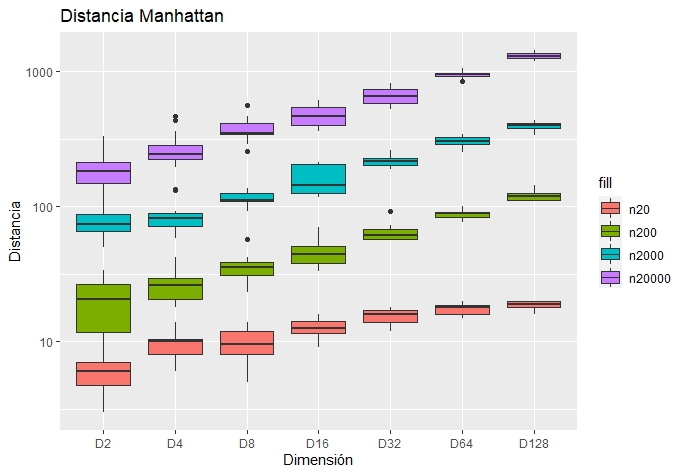
\includegraphics[width=170mm]{Figura3.jpeg} % archivo
    \caption{Segundo intento de diagrama caja-bigote importando datos desde un archivo de Excel.}
    \label{Figura3}
\end{figure}

Finalmente me base en el codigo ejemplo de la Dra. Elisa para realizar un data.frame debidamente ordenado, además entendí como realizar la secuencia de las 4 caminatas sin tener que poner 4 'for' como lo estaba haciendo. 

El codigo final para obtener el Diagrama caja-bigote de acuerdo al objetivo de la practica se muestra a continuacion:

\begin{lstlisting}

library(dplyr) 
library(ggplot2) #libreria para graficar boxplot agrupado
library(scales) #libreria para hacer modificaciones a la grafica
datos = data.frame() #para almacenar los datos obtenidos
niveles = c(20, 200, 2000, 20000) #caminatas: Nivel 1, Nivel 2, Nivel 3 y Nivel 4

for (dimension in c(2**1, 2**2, 2**3, 2**4, 2**5, 2**6, 2**7)) { #seleccionar dimension
  for (duracion in niveles) { #seleccionar la caminata
    for (replica in 1:12) { #repetir el experimento
      pos = rep(0, dimension)
      mayor = 0
      for (t in 1:duracion) {
        cambiar = sample(1:dimension, 1)
        cambio = 1
        if (runif(1) < 0.5) {
          cambio = -1
        }
        pos[cambiar] = pos[cambiar] + cambio
        d <- sum(abs(pos))
        
        
        
        if (d > mayor) {
          mayor = d
        }
      }
      resultado <- c(dimension, duracion, replica, mayor) #vector para agrupar resultados
      datos <- rbind(datos, resultado) #para llenar en el dataframe vacio
    }
  }
}
names(datos) <- c("dim", "Caminata", "rep", "dist") #nombrar columnas del dataframe 

datos$dim = as.factor(datos$dim) #crear vector a partir del dataframe
datos$Caminata = as.factor(datos$Caminata) #crear vector a partir del dataframe

ggplot(datos, aes(x= dim, y= dist, fill= Caminata)) + 
  geom_boxplot(width=1)+
  labs(x = "Dimension", y = "Distancia", title = 'Distancia Manhattan')+ #nombres
  scale_y_log10() #cambiar la escala del eje "y" a logaritmo

\end{lstlisting}
\bigskip

El Diagrama caja-bigote que se obtiene del codigo anterior para 4 caminatas diferentes (Nivel 1= 20, Nivel 2= 200, Nivel 3 = 2000, Nivel 4 = 20000, con 2, 4, 8, 16, 32, 64 y 128 dimensiones y repitiendo el experimento 12 veces, se muestra en la Figura 4.

\begin{figure}[h!]% figura
    \centering
    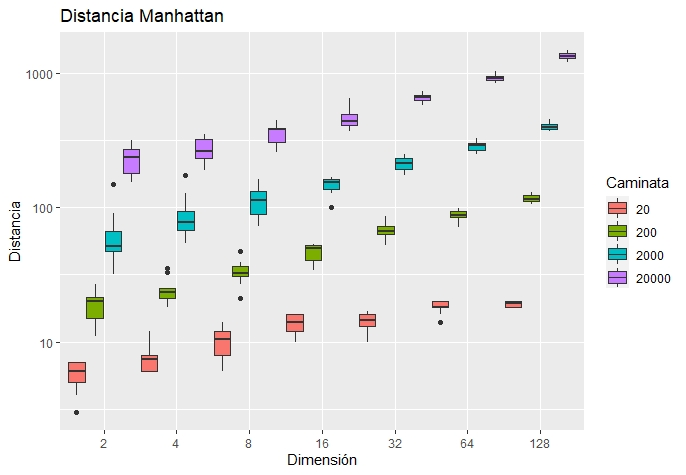
\includegraphics[width=170mm]{Figura4.jpeg} % archivo
    \caption{Diagrama caja-bigote con el eje y 'Distancia' en escala log10.}
    \label{Figura4}
\end{figure}

\newpage
.
\bigskip
\bigskip

\begin{figure}[h!]% figura
    \centering
    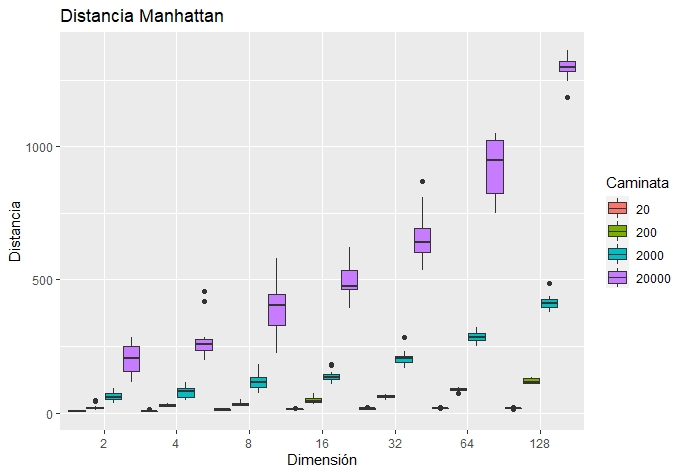
\includegraphics[width=170mm]{Figura5.jpeg} % archivo
    \caption{Diagrama caja-bigote sin escala en el eje y.}
    \label{Figura5}
\end{figure}

\bigskip

\section{Conclusi\'{o}n}
Con base en los resultados que se muestran en los Diagramas Caja-bigote de la Figura 4 y Figura 5 se puede concluir que al aumentar la cantidad de dimensiones en que se puede mover la partícula la distancia que recorre es mayor, considero que esto se debe a que tiene un mayor espacio para moverse y existe menos probabilidad de que regrese al origen. También se puede notar que cuando se aumenta el número de pasos de la caminata de la partícula se tiene un rango de distancias mayor.

\bigskip

En general el desarrollo de la práctica me permitió explorar más a fondo las funciones que tiene el programa RStudio, además de familiarizarme con su interfaz y también obtuve más práctica con el programa Overleaf. Así mismo considero que aún tengo mucho que aprender en cuanto a programación de código, dado que tuve muchas dificultades en esa parte.

\newpage
.
\bigskip
\bigskip

\bibliography{referencias}
\bibliographystyle{plainnat}

\end{document}